\documentclass{sigchi}

% Use this section to set the ACM copyright statement (e.g. for
% preprints).  Consult the conference website for the camera-ready
% copyright statement.

% Copyright
\CopyrightYear{2019}
%\setcopyright{acmcopyright}
\setcopyright{acmlicensed}
%\setcopyright{rightsretained}
%\setcopyright{usgov}
%\setcopyright{usgovmixed}
%\setcopyright{cagov}
%\setcopyright{cagovmixed}
% DOI
\doi{http://dx.doi.org/10.475/123_4}
% ISBN
\isbn{123-4567-24-567/08/06}
%Conference
\conferenceinfo{UIST'19,}{October 20--23, 2016, New Orleans, LA, USA}
%Price
\acmPrice{\$15.00}

% Use this command to override the default ACM copyright statement
% (e.g. for preprints).  Consult the conference website for the
% camera-ready copyright statement.

%% HOW TO OVERRIDE THE DEFAULT COPYRIGHT STRIP --
%% Please note you need to make sure the copy for your specific
%% license is used here!
% \toappear{
% Permission to make digital or hard copies of all or part of this work
% for personal or classroom use is granted without fee provided that
% copies are not made or distributed for profit or commercial advantage
% and that copies bear this notice and the full citation on the first
% page. Copyrights for components of this work owned by others than ACM
% must be honored. Abstracting with credit is permitted. To copy
% otherwise, or republish, to post on servers or to redistribute to
% lists, requires prior specific permission and/or a fee. Request
% permissions from \href{mailto:Permissions@acm.org}{Permissions@acm.org}. \\
% \emph{CHI '16},  May 07--12, 2016, San Jose, CA, USA \\
% ACM xxx-x-xxxx-xxxx-x/xx/xx\ldots \$15.00 \\
% DOI: \url{http://dx.doi.org/xx.xxxx/xxxxxxx.xxxxxxx}
% }

% Arabic page numbers for submission.  Remove this line to eliminate
% page numbers for the camera ready copy
% \pagenumbering{arabic}

% Load basic packages
\usepackage{balance}       % to better equalize the last page
\usepackage{graphics}      % for EPS, load graphicx instead 
\usepackage[T1]{fontenc}   % for umlauts and other diaeresis
\usepackage{txfonts}
\usepackage{mathptmx}
\usepackage[pdflang={en-US},pdftex]{hyperref}
\usepackage{color}
\usepackage{booktabs}
\usepackage{textcomp}

% Some optional stuff you might like/need.
\usepackage{microtype}        % Improved Tracking and Kerning
% \usepackage[all]{hypcap}    % Fixes bug in hyperref caption linking
\usepackage{ccicons}          % Cite your images correctly!
% \usepackage[utf8]{inputenc} % for a UTF8 editor only

% If you want to use todo notes, marginpars etc. during creation of
% your draft document, you have to enable the "chi_draft" option for
% the document class. To do this, change the very first line to:
% "\documentclass[chi_draft]{sigchi}". You can then place todo notes
% by using the "\todo{...}"  command. Make sure to disable the draft
% option again before submitting your final document.
\usepackage{todonotes}

% Paper metadata (use plain text, for PDF inclusion and later
% re-using, if desired).  Use \emtpyauthor when submitting for review
% so you remain anonymous.
\def\plaintitle{Loveform: the generative design of sculptural forms from spoken word}
\def\plainauthor{Hye Yeon Nam, Brendan Harmon}
\def\emptyauthor{}
\def\plainkeywords{Geovisualization; climate change; sea level rise; robotics.}
\def\plaingeneralterms{Design, Human Factors}

% llt: Define a global style for URLs, rather that the default one
\makeatletter
\def\url@leostyle{%
  \@ifundefined{selectfont}{
    \def\UrlFont{\sf}
  }{
    \def\UrlFont{\small\bf\ttfamily}
  }}
\makeatother
\urlstyle{leo}

% To make various LaTeX processors do the right thing with page size.
\def\pprw{8.5in}
\def\pprh{11in}
\special{papersize=\pprw,\pprh}
\setlength{\paperwidth}{\pprw}
\setlength{\paperheight}{\pprh}
\setlength{\pdfpagewidth}{\pprw}
\setlength{\pdfpageheight}{\pprh}

% Make sure hyperref comes last of your loaded packages, to give it a
% fighting chance of not being over-written, since its job is to
% redefine many LaTeX commands.
\definecolor{linkColor}{RGB}{6,125,233}
\hypersetup{%
  pdftitle={\plaintitle},
% Use \plainauthor for final version.
  pdfauthor={\plainauthor},
%  pdfauthor={\emptyauthor},
  pdfkeywords={\plainkeywords},
  pdfdisplaydoctitle=true, % For Accessibility
  bookmarksnumbered,
  pdfstartview={FitH},
  colorlinks,
  citecolor=black,
  filecolor=black,
  linkcolor=black,
  urlcolor=linkColor,
  breaklinks=true,
  hypertexnames=false
}

% create a shortcut to typeset table headings
% \newcommand\tabhead[1]{\small\textbf{#1}}

\begin{document}

\title{\plaintitle}

\numberofauthors{3}
\author{%
  \alignauthor{Hye Yeon Nam\\
    \affaddr{Louisiana State University}\\
    \affaddr{Baton Rouge, USA}\\
    \email{hyenam@lsu.edu}}\\
  \alignauthor{Brendan Alexander Harmon\\
    \affaddr{Louisiana State University}\\
    \affaddr{Baton Rouge, USA}\\
    \email{baharmon@lsu.edu}}\\
}

\maketitle

\begin{abstract}
%150 words
\end{abstract}

\category{H.5.1.}{Information Interfaces and Presentation
  (e.g. HCI)}{Multimedia Information Systems}
\category{J.5}{Arts and Humanities}{Fine Arts}

\keywords{Generative design, tangible interaction; digital fabrication.}
% 3D printing

\section{Introduction}

Loveform is a way to share personal messages in an abstract physical form with audio triggered on interaction. It is an interactive, 3D printed ceramic cup derived from the waveform of a spoken message that recites its recorded message when drunk from.  Our first pair of cups each represent and recite the message `I love you' (Figure~\ref{fig:loveform_1}). Loveform is about tangible interaction with abstract physical representations of audio. The cups and saucers function as a tangible interface for playing encoded messages. Precedents for the generative design include Nervous Systems’ Coral Cup and Porifera jewelry collection \cite{NervousSystem2018,NervousSystem2018a} and for the simple tangible interaction include Durrell Bishop's Marble Answering Machine \cite{Dragicevic2014} and Philip's Mindspheres \cite{Djajadiningrat2008}. Using our open source software, users can record their own messages and generate unique cups for 3D printing. Code for this project is available at \url{https://github.com/baharmon/waveforms} under the  Creative Commons Attribution-ShareAlike 4.0 International (CC BY-SA 4.0) license.

\begin{figure*}
  \centering
  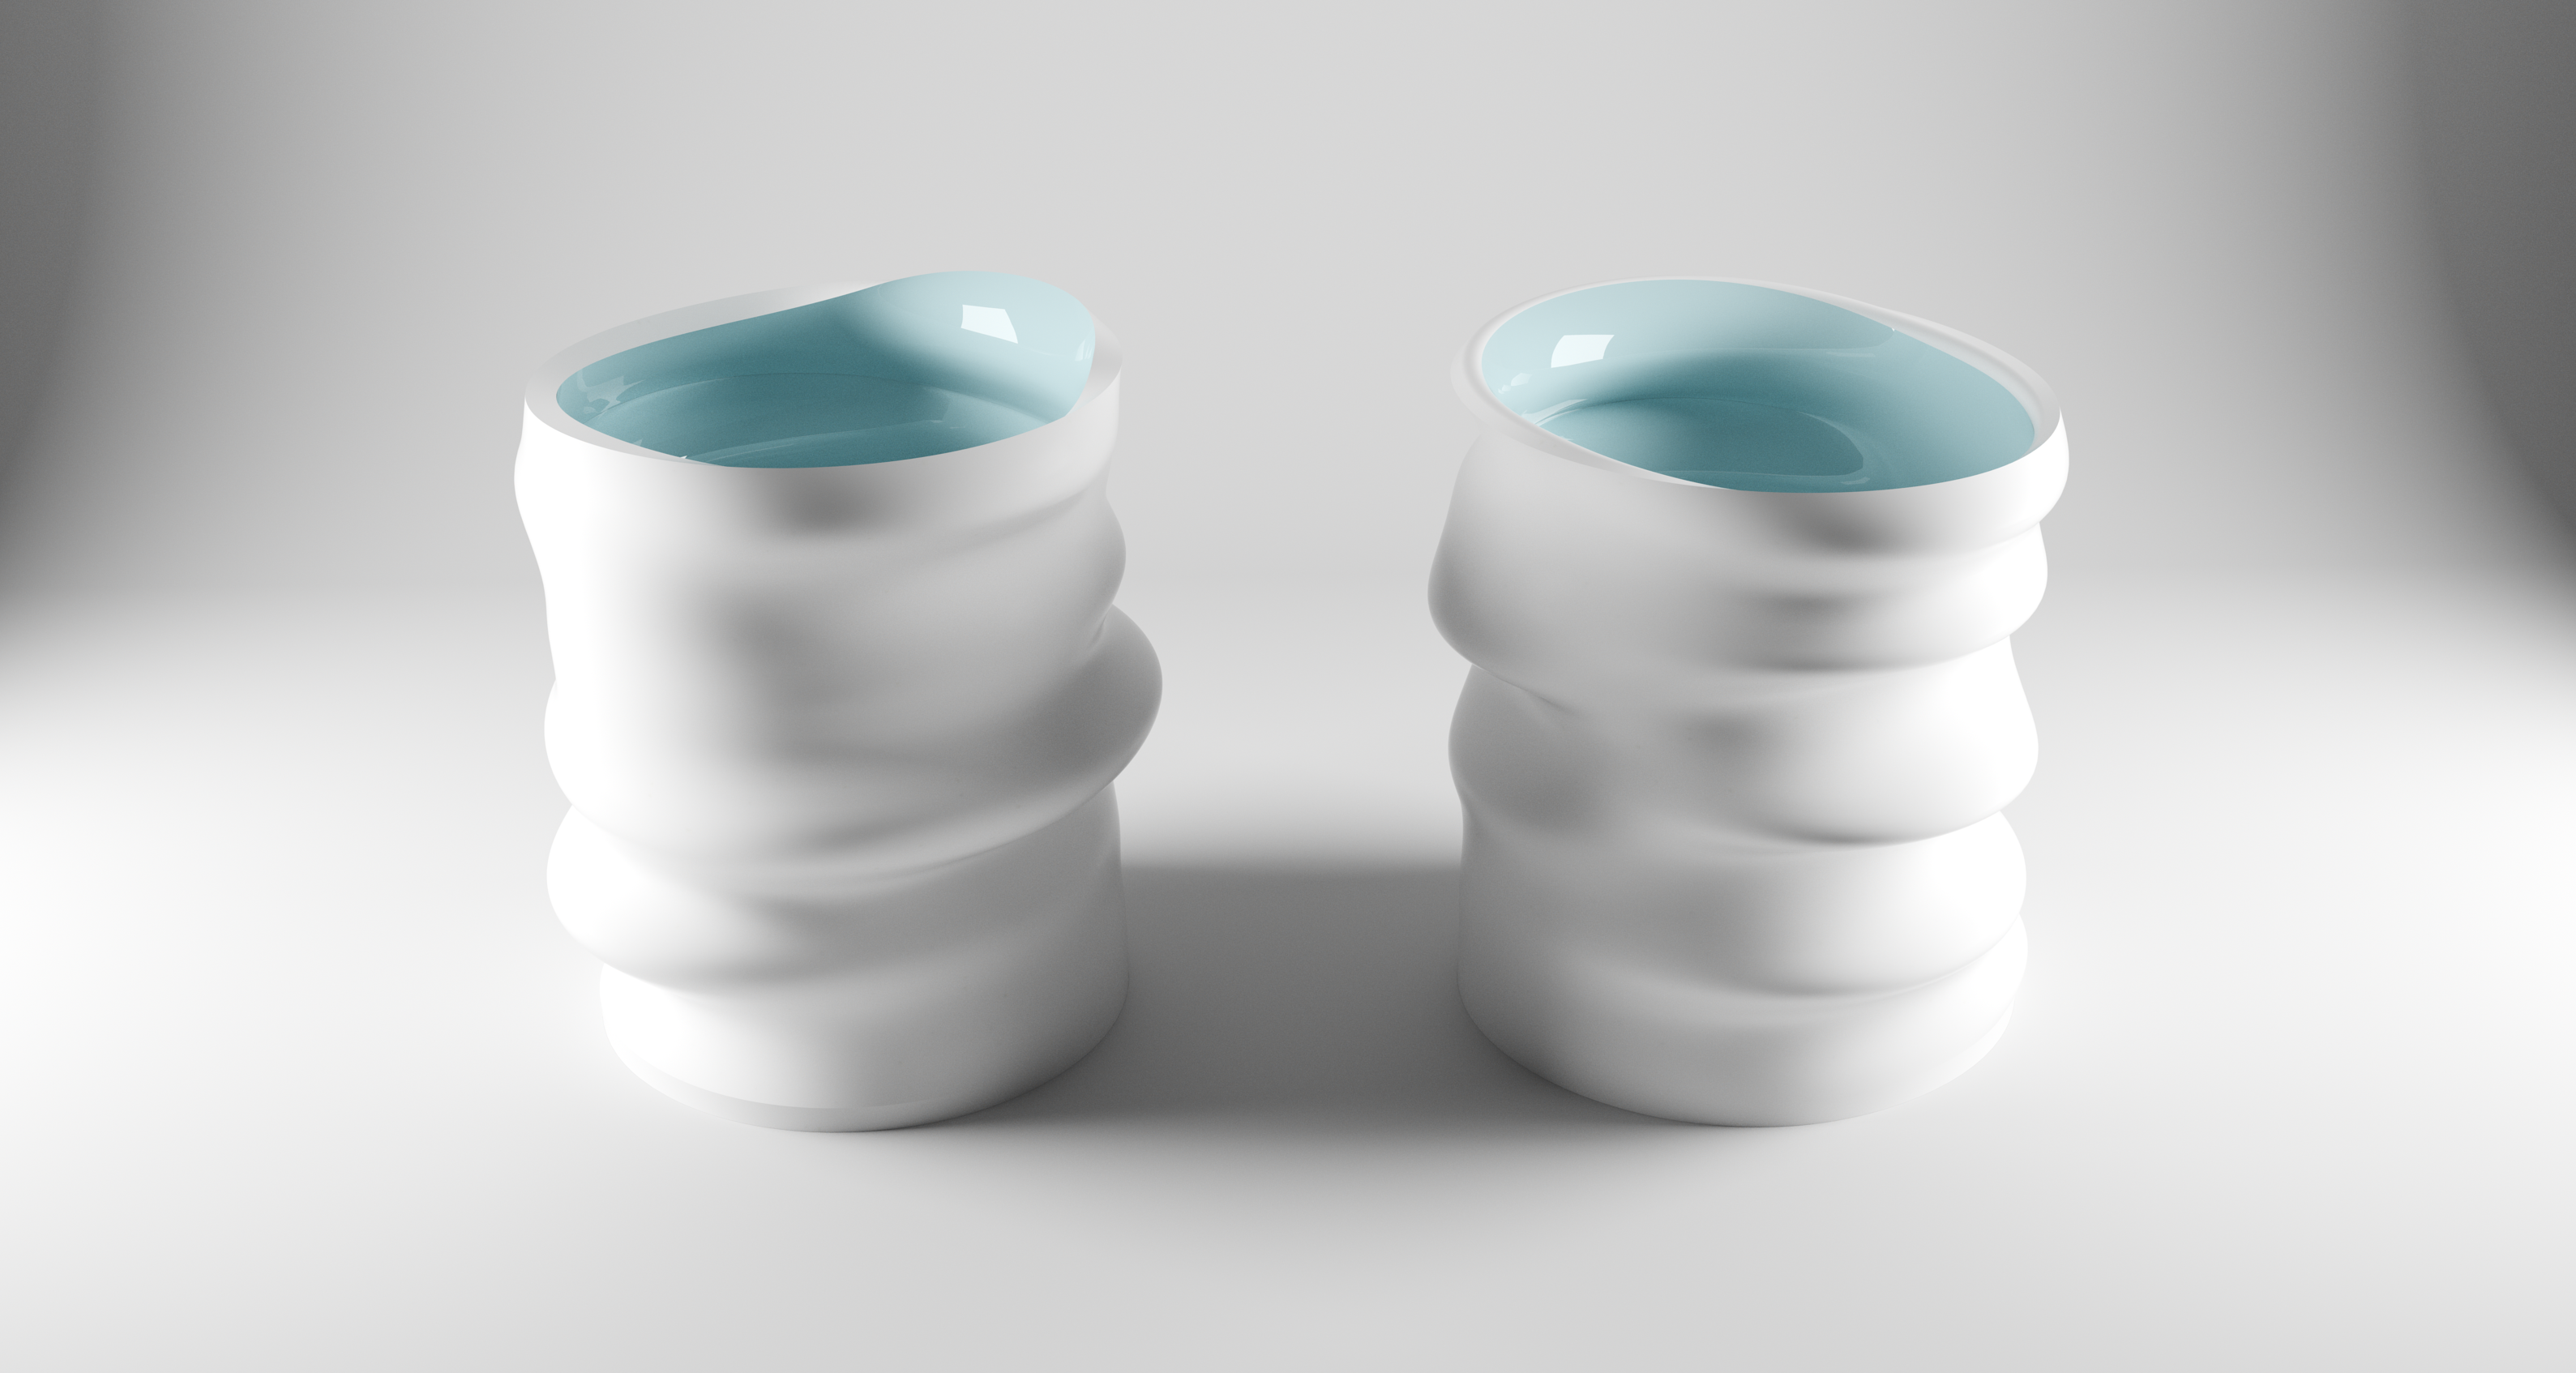
\includegraphics[width=2.0\columnwidth]{../../images/loveform-thea-rendering-2.png}
  \caption{Loveform, 3D printed ceramic cups}~\label{fig:loveform_1}
\end{figure*}

\section{Generative design and fabrication}
We each recorded our message -- `I love you' -- and used Grasshopper,  Rhinoceros 3D's visual programming language, to parametrically model the waveforms of each recording as sculptural forms. Our Grasshopper script draws the waveform of a recording as a curve, divides this curve into segments, translates and rotates these segments around a circle, sweeps the segments into a surface, and then extrudes the surface into a volume. Once we had generated the models,  we 3D printed plaster negatives of the cups as formwork and then slip cast, bisque fired, glazed, and then fully fired the cups. We also experimented with 3D printing the cups with a ceramic resin. 

\section{Tangible interaction}
While each cup's sculptural form physically represents the unique waveform of the message it encodes, drinking from the cup plays back the encoded message as audio. Each cup rests on a saucer – an epoxy cast of a cupped hand embedded with a sensor, microcontroller, and speaker – that can playback the encoded message. When a cup is picked up to be drunk from, its saucer will play back the message that the cup represents. Picking up the cup releases pressure on a pressure sensor, triggering the recording to play. A tactile transducer generates the sound by vibrating the saucer. Users can record their our messages by whispering their own secrets into an epoxy cast of an ear embedded with a recording device. Each secret will be recorded, parametrically modeled as a sculptural vessel, and saved as a stereolithography file for 3D printing. Users can take their stereolithography files to a makerspace or use an online service like Shapeways for 3D printing.  








\section{Conclusion}

\ldots

\section{Acknowledgments}
\ldots

\balance{}

% BALANCE COLUMNS
\balance{}

% REFERENCES
\bibliographystyle{SIGCHI-Reference-Format}
\bibliography{references}

\end{document}

%%% Local Variables:
%%% mode: latex
%%% TeX-master: t
%%% End:
